\newpage
\section{Calculation and Simulation} %  of Rolling Roads regulator
\label{sec:Calculation_and_Simulation}

This section will go though the simulation of Rolling Roads regulator. First what kind of regulator what has been choose for the Rolling Road and then the calculation of regulator and finally a simulation too see if it will work.

\subsection{Calculation}

PID regulator, because it the most common used regulator.

Before the constants of the PID regulator can be chosen, The transfer function of the load system has to be found first.

The load system consists of some elements: A generator that both have a resistor and a inductor. A Power Mosfet what is control by a PWM signal, as a approximation just calculate it as a gain. It has a load part with a power resistor.

All result are calculate with Matlab. Script (RollingRoad.m)   

A list of all constants what are used.
\lstset{language=MATLAB}
\begin{lstlisting}
	%% Constants
	L_a      = 0.000072;        %DC-generator inductance (H)
	R_a      = 0.103;           %Anchor resistance (Ohm)
	R_load   = 1.1;             %Load resistance (Ohm)
	Kt       = 38.5*10^(-3);    %Torque Constant (Nm/A)
	Gear     = 4.3;             %Gearing ratio in the motor
	RR_r     = 0.076            %RollingRoad radius (m)
	Kb       = Kt;              %Speed constant (rpm/Nm)
	M_t      = 0.00378          %Motor time constant. (s)
	K_pwm    = 256;             %PWM steps 
	Moment_fc= 178.6251			%Torque sensor filter cut frequency(rad/s)
	
	% Convert 
	OmegaToRpm = 60/(2*pi);
	SpeedToOmega = (2*pi)/(2*pi*RR_r);
	SpeedToRpm = SpeedToOmega * OmegaToRpm;
	Km_hTom_s = 1000/3600;
	KmToRpm=Km_hTom_s*SpeedToRpm
\end{lstlisting} 

Calculations of the load system:

\begin{lstlisting}
	%%% transfer functions
	
	% transfer function of the generatoren.
	T_generator=tf((1/M_t)/(s+(1/M_t))) % motor delay
	
	% transfer function for Moment/rpm.
	Ea=tf(T_generator*Gear*Kb*Kt/(R_a+R_load)) % Moment/rpm    //
	
	% at a steady speed.
	TT=Ea*V_rpm % if speed is not constant have to add an extra T_generator
	
	% note because the speed affects proportional on the system. there be
	% something there adjusted receptional of the speeds proportional affect.
	% This can be done with a function of speed
	
	syms v_rpm
	
	P_rpm=1/(v_rpm*Gear*Kb*Kt/(R_a+R_load))
	% must be implemented into the code.
	
	func_P=(V_rpm*Gear*Kb*Kt/(R_a+R_load))^-1
	
	Ggenerator=tf(func_P*TT)
	
	% PWM signal transfer function 
	
	G_PWM=(1/K_pwm)
	
	% Torque sensor filter
	
	G_moment_filter=(Moment_fc*2*pi) / (s + Moment_fc*2*pi)
	
	% total transfer function of the plant.
	
	Gplant = G_PWM*Ggenerator
	
	% Open loop bode
	Gplant*G_moment_filter
	figure
	bode(Gplant*G_moment_filter)
	grid on
	legend('show')
\end{lstlisting} 

\begin{figure}[H]
	\centering
	\includegraphics [width=4in]{Hardware/Pictures/RolingRoad_01.eps}
	\caption{Open loop bode plot of the load system}
	\label{fig:Open_loop_bode_load_system}
\end{figure}

\ref{fig:Open_loop_bode_load_system} are a open loop response from the load system, and it this bode plot what are used to determine the PID constants.

First step is to find the wanted Phase margin and the minimum Omega bandwidth. Then the requirements is OS 5 \% and settling time is max 100 ms.

\newpage

\begin{lstlisting}
	%% Calculation of PID constanst
	% requirements
	
	Ts=0.1;
	
	OS=5; 
	
	% Calculation
	
	Zeta = (-log( OS / 100 ))/(( pi^2 + log( OS / 100 )^2)^0.5)
	
	Phase_m = atan( ( 2 * Zeta ) / (( -2 * Zeta^2 + ( 1 + 4 * Zeta^4)^0.5 )^0.5))*(180/pi) + 7
	
	Omega_BW_min = ( 4 / ( Zeta * Ts )) * sqrt(( 1 - 2 * Zeta^2 ) + sqrt( 4 * Zeta^4 ) - 4 * Zeta^2 + 2 ) 
\end{lstlisting} 

And the result are fund, and now it is just to find have much gain there is needed to get this $ \phi_{m} $. And find the $ \omega _{\phi _{m}} $ to determine the value of the "I" part. If the $ \omega _{\phi _{m}} $ is too small a "D" part is also needed. 

\begin{equation}
	\begin{split}
		\phi_{m}= 71.6 + ( -7 )\\
		\omega_{{BW}_{{min}}}= 60.7
	\end{split}
\end{equation}

The values for the PID regulator is: 

\begin{equation}
	\begin{split}
		P = 1035.1\\
		I = 81.6\\
		\omega _{\phi _{m}}=816\\
		P_{{rpm}} \left( v_{{rpm}} \right) = \frac{188.7}{v_{{rpm}}}
	\end{split}
\end{equation}

Note there is no need for a "D" part because the PI regulator is fast enough ($ \omega _{\phi _{m}} > \omega_{{BW}_{{min}}} $ ). There is and extra "P" ($ P_{{rpm}} \left( v_{{rpm}} \right) $) part this is just to adjusted for the speed.


\begin{figure}[H]
	\centering
	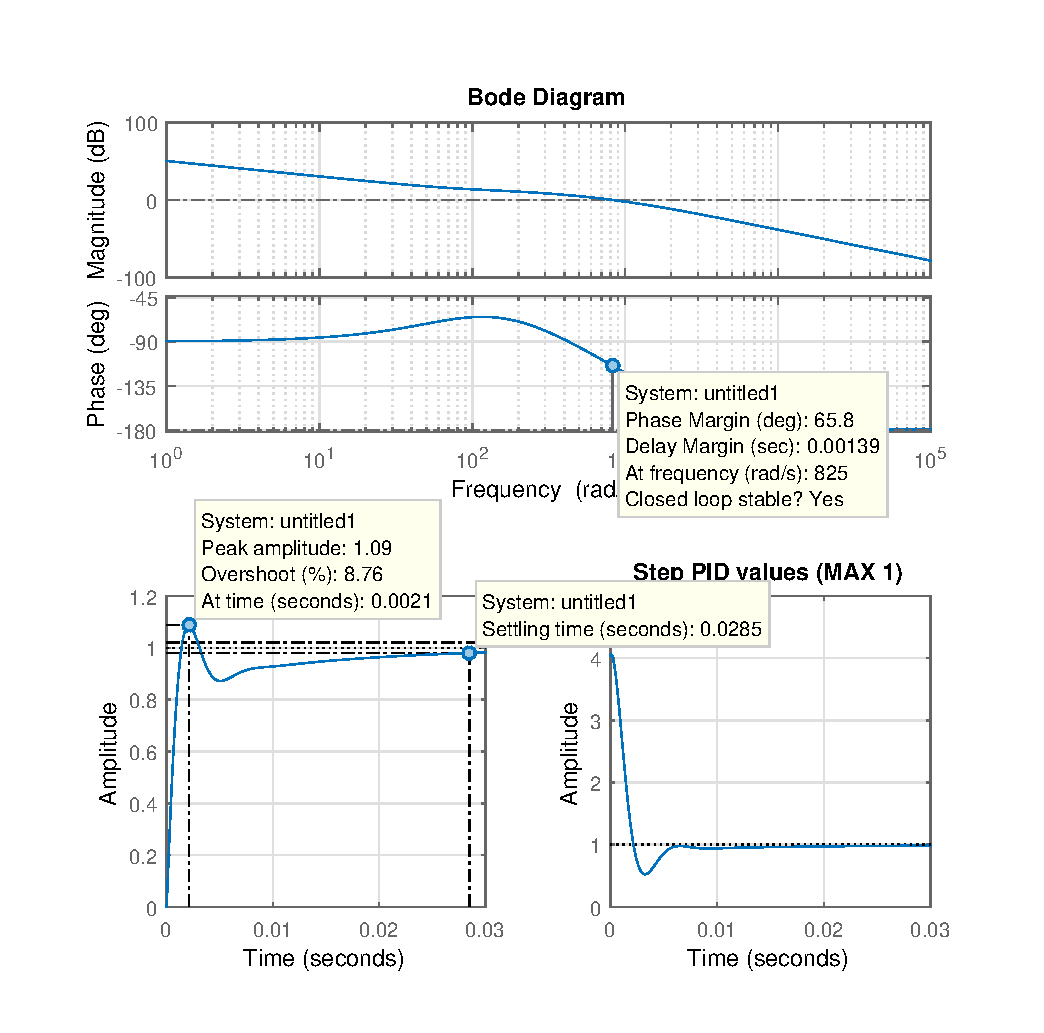
\includegraphics [width=6in]{Hardware/Pictures/RolingRoad_PI_result.eps}
	\caption{Open loop bode plot, close loop step of the load system with PI regulator}
	\label{fig:Open_loop_bode_close_loop_step_load_system}
\end{figure}

In \ref{fig:Open_loop_bode_close_loop_step_load_system} there are three plots, the "Bode Diagram" is the open loop plot of the load system and the PI regulator, it seems like it should be alright, but in the step response to the left, there are $ 8.8 \% $ OS this it not good. But the settling time is more then 3 times smaller when required. Where is one more thing what is gonna be a problem, see on the right step response (It a step response of PID values), because it is a PWM signal, it can max be 1!. So the PI regulator are saturate, this will make the settling time slower in the real life. 

There is just one thing left again, the PI regulator is in site of a PSoC 5LP, and therefor it is a digital regulator. First step in this conversion is to find a good sampling time. The sampling time is determined by Åstrøm and Wittenmark:

\begin{equation}
\begin{split}
	\frac{0.15}{\omega _{\phi _{m}}} \leq T_{s} \leq \frac{0.5}{\omega _{\phi _{m}}}\\
	Ts_{max} = 6.1275 \times 10^{-4}\\
	Ts_{min} = 1.8382 \times 10^{-4}\\
	Fs_{max} = 5440\\
	Fs_{min} = 1632
\end{split}
\end{equation}

\begin{figure}[H]
	\centering
	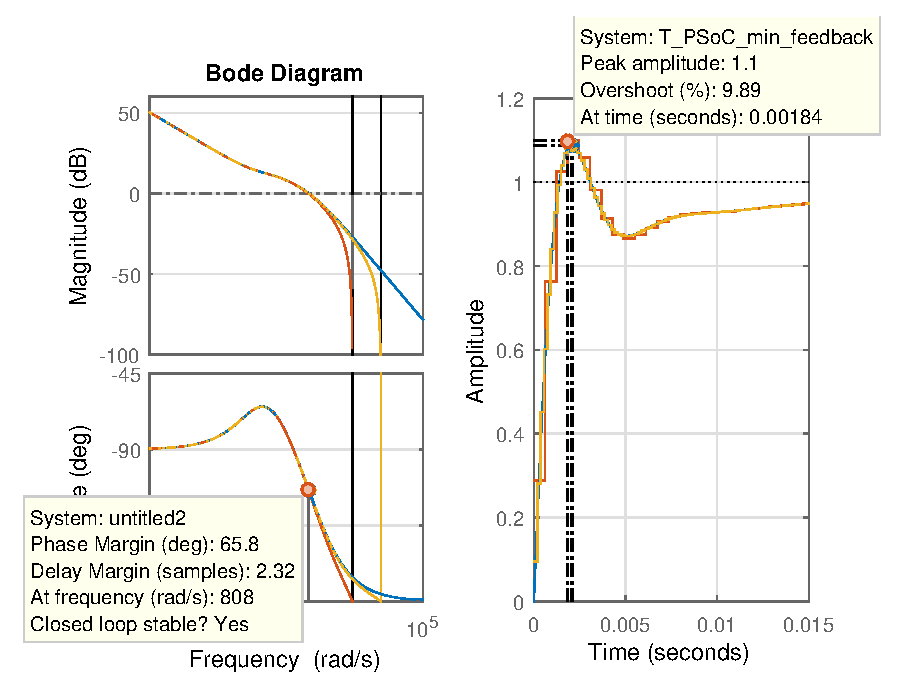
\includegraphics [width=6in]{Hardware/Pictures/RolingRoad_PI_PSOC_result.eps}
	\caption{Open loop bode plot, close loop step of the load system with PI on a PSoC 5LP regulator}
	\label{fig:Open_loop_bode_close_loop_step_load_system_PSOC}
\end{figure}

So there should not be any problem to use the PSoC as long as PI regulator samples around $ 2000  \frac{Sample}{s} $.

\newpage
\subsection{Simulation}

Before making the Rolling Road a simulation of the system was made, to check that the theory was right. To do this task Matlab Simulink was used.

\begin{figure}[H]
	\centering
	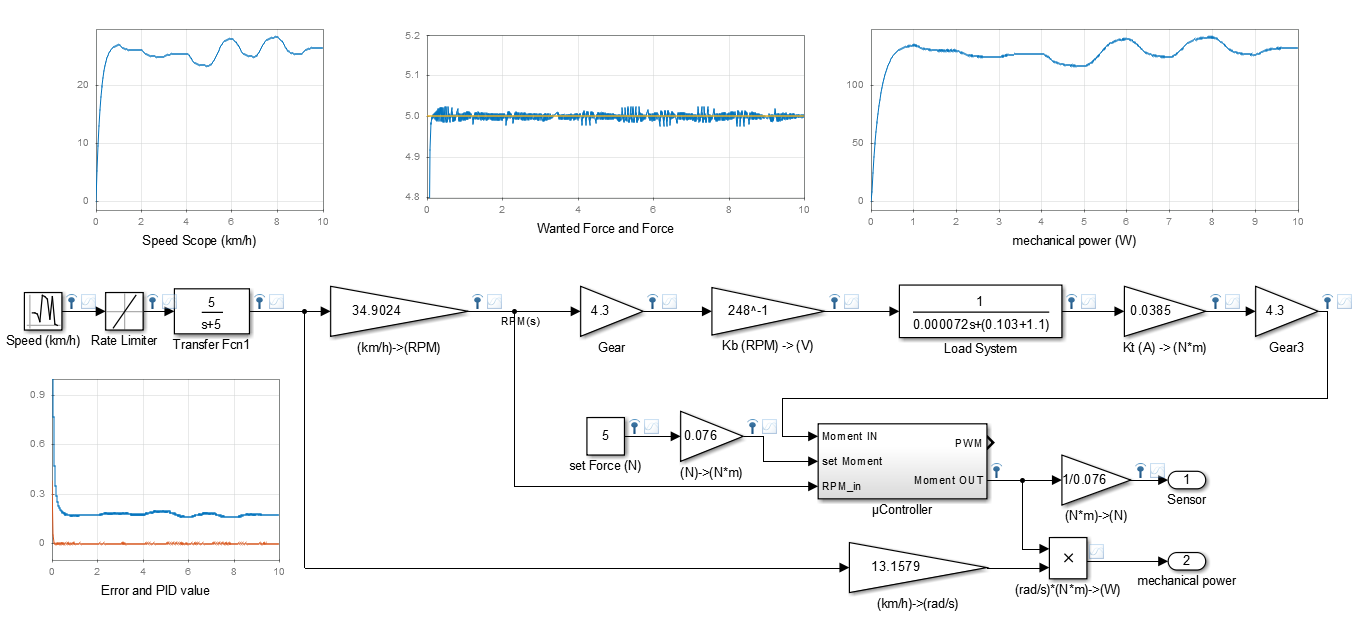
\includegraphics [width=6in]{Hardware/Pictures/simulation_top.PNG}
	\caption{Simulation model: top model}
	\label{fig:sim_top}
\end{figure}

The top model in \ref{fig:sim_top} are a simulation of how the speed of a moving object will produce a reverse force on it self then using the Rolling Road. Of course the Rolling Road can control how much force that will be send back to the test object.\\
The first block on the left side "Speed (km/h)" are the speed that the test object runs with. The next two block are only used to make a more smooth speed curvy.\\
The next thing what happening is that the speed are been convert to a rotational speed.\\
Before the generator is there a Gear, and the rotating speed goes up.\\
The next 3 blocks are the transformation in generator and load system, where the speed are converted to a torque.\\
The torque are control with a PID regulator (see \ref{fig:sim_PSOC}). of course this part are controlling the current and not the torque, but it the same just a different scale. So just to get better overview it will seem as it the torque that are been regulated and not the current.\\ 
After the PID regulator has regulated the torgue, the torque are send back to the object and are converted to a force.   

\begin{figure}[H]
	\centering
	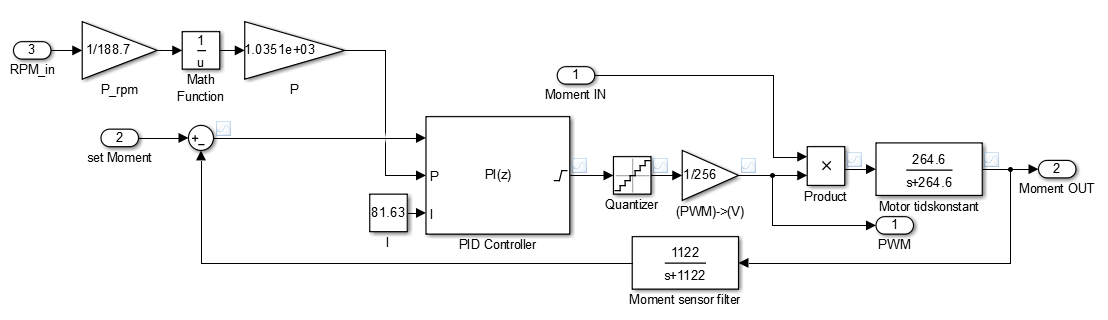
\includegraphics [width=6in]{Hardware/Pictures/simulation_uController.PNG}
	\caption{Simulation model: µController}
	\label{fig:sim_PSOC}
\end{figure}  

This is the digital PID regulator \ref{fig:sim_PSOC}, the special thing with the regulator is that it has a function of rotational speed to the propagation part. Sample frequency is set to 2000 S/s. The PID regulator are controlling a Power Mosfet wish is the same as a Product in the simulation. It is also this part that is the reason the Propagation part need to be a function of rotational speed. after it has been regulated where is a little time delay from the power circuit too the mechanical part, in the feedback loop are there also implemented a anti-aliasing filter for the torque sensor.  
